\documentclass[Dissertation.tex]{subfiles}
\begin{document}

\chapter{Background and Literature Review}
This chapter contains a review of previously written academic literature in topics related to the project aims and objectives. The chapter begins with an exploration of the meaning of stance both in everyday language and in academia to introduce the concept to readers with no formal education in linguistics.  Following this, topics in machine learning are examined provide context for both section \ref{stanceDetection}, which reviews existing research related to stance detection, and section \ref{designAndBuild}, which describes the models and experiments used in this project. Finally, the chapter concludes with a review of the Brexit Blog Corpus by Simaki et al.\ \cite{simakiAnnotatingSpeakerStance2017}, which is the principle dataset for this project.
 
\section{Speaker Stance in Linguistics}\label{sec:speakerStanceLing}
To begin with, the notion of speaker stance must be conceptualised and explored to broadly inform the remainder of this project. There exists a wealth of contemporary linguistic research pertaining to stance. A number of textbooks and monographs have been published explicitly devoted to stance and stancetaking
\cite{hunstonEvaluationTextAuthorial2000}, \cite{englebretsonStancetakingDiscourseSubjectivity2007},\cite{karkkainenEpistemicStanceEnglish2003}, 
%
% consider revising below
conferences have been hosted to bring together researchers in the field
%
%
and  many journal articles from different subfields in linguistics have converged upon the topic [CITATION NEEDED]. This heterogeneous body of research demonstrates a marked interest in developing understanding of stance, however it also demonstrates that stance is a broad and nuanced topic, with no universally agreed upon definition in academia. This section closely follows the work of Englebretson \cite{englebretsonStancetakingDiscourseSubjectivity2007} in order to present an overview of linguistic perspectives on stance.

To begin with, it is useful to examine the colloquial usage of the term \textit{stance} in natural language, since this can offer insight into the ways in which its meaning has been appropriated by the linguistic research community \cite{englebretsonStancetakingDiscourseSubjectivity2007}. This approach is known as a usage-based perspective of language, which asserts that language form and meaning can be best understood by examining language use, as opposed to understanding language through rule based systems \cite{barlowUsagebasedModelsLanguage2000}. 

The Oxford Dictionary of English  \cite{StanceOxfordReference} defines the noun stance to mean:

\begin{displayquote}
	\begin{enumerate}
		\item the way in which someone stands, especially when deliberately adopted.
		\item the attitude of a person or organization towards something; a standpoint.
	\end{enumerate}
\end{displayquote}

This definition provides a useful starting point. Note that stance is defined as referring either to a physical orientation or a subjective outlook - this is the foundation of most linguistic characterizations of stance. Investigating in more detail the properties of the term and the contexts in which it appears further assists the construction of academic definitions of speaker stance. Englebreston \cite{englebretsonStancetakingDiscourseSubjectivity2007} presents a corpus based quantitative and qualitative analysis of the usage of the term stance in colloquial language. The analysis identifies five key principles that describe stance, which we will examine in detail in this section. Consider the following sentences, inspired by entries examined in the corpus analysis \cite{englebretsonStancetakingDiscourseSubjectivity2007}:


\begin{enumerate}
	\renewcommand{\labelenumi}{(\Alph{enumi})}
	\item `The fighter took a defensive stance'
	\item `He was known amongst his peers for his conservative political stance'
	\item `Young people are leaving the Catholic Church due to its moral stance on abortion'
	\
\end{enumerate}

The five key principles identified by Englebretson \cite{englebretsonStancetakingDiscourseSubjectivity2007} are:
\begin{enumerate}
	\item Stancetaking can occur in three overlapping ways - as a physical action, a personal attitude or a social value. (A) clearly demonstrates the physical sense of \textit{stance}, while (B) shows it as a personal attitude, and in (C) we see it can indicate a social value (morality). 
	
	\item Stance is public, interpretable and available to for inspection by others. For example, in (A) the fighter's opponent can notice the defensive stance, while in example (B) the subject's peers have assessed his political stance to be a key aspect of his character.
	
	\item Stance is interactional in nature - it cannot exist in a vacuum. In (A) the  phrase \textit{defensive stance} refers to the fighters positioning in against his opponent, while in (C) the Church's stance is in opposition of those in favour of abortion. Without the notional `other', the stances do not make sense.
	
	\item Stance is indexical, i.e. the context in which \textit{stance} is used can point towards other unmentioned attributes. For example, in (B) the conservative political stance implicitly 'indexes' the subject as holding certain views  associated with conservatism, and also implies that his peers do not. Similarly, in (C) the categorization of their stance as `moral' implicitly suggests that the Church disagrees with abortion.
	
	\item Stance is consequential. In (A) the fighter may find it harder to attack his opponent due to his defensive stance, while in (B) the subject has been labelled by his peers for his stance, and (C) explicitly states a consequence of the Church's stance on abortion.
\end{enumerate}

Engelbretson \cite{englebretsonStancetakingDiscourseSubjectivity2007} further justifies these five principles by quantitative analysis of the corpora. A key observation is that the term \textit{stance} is a relatively rare lexeme generally that appears far more frequently in written text than in spoken language. This suggests that \textit{stance} is a term that appears mostly in specialized contexts. These contexts are demonstrated by examining the adjective collocates of \textit{stance} \cite{englebretsonStancetakingDiscourseSubjectivity2007}. The five most common adjectives thereby are \textit{political, aggressive, moral, upright} and \textit{tough}. These five adjectives broadly speaking support the aforementioned five principles. For example, \textit{political} and \textit{moral} exemplify stance as a personal attitude or social value, while \textit{upright} demonstrates the physicality of stance. Finally, \textit{tough} and \textit{aggressive} can be interpreted in all three contexts. CONTINUE OR RAP UP

%%Consider extending quantitative justifications

Having considered qualitative and quantitative perspectives on the usage of stance we can see that the term has many contexts and definitions.  It is therefore consistent that the appropriation into academic contexts of stance comes in many forms, with different researchers invoking varying practical definitions of speaker stance.

Critical to understanding such definitions of stance are \textit{subjectivity} and \textit{evaluation}. Subjectivity is the aspect of language that allows interlocutors (speakers)  to express themselves and describe their own point of view, for example using the pronouns \textit{I} and \textit{Me} \cite{matthewsSubjectivity2014}. Evaluation is the expression of subjective sentiment concerning an entity or proposition, such as expressing an attitude or opinion \cite{hunstonEvaluationTextAuthorial2000}. These two concepts are relied upon heavily by Biber and Finegan \cite{biberStylesStanceEnglish1989}, which defines stance as:

\begin{displayquote} `` The lexical and grammatical expression of attitudes, feelings, judgments, or commitment concerning the propositional content of a message ''
\end{displayquote}


Furthermore, Biber and Finegan \cite{biberStylesStanceEnglish1989} identifies twelve groups of stance markers (such as certainty verbs or predictive modals) based on semantic and grammatical criteria. Using cluster analysis of corpora using these stance markers, they identify six separate styles of stance, such as ‘Emphatic Expression of Affect’ and ‘Expository Expression of Doubt’ \cite{biberStylesStanceEnglish1989}. 

In a similar fashion Simaki et al.\ \cite{simakiAnnotatingSpeakerStance2017} (which this project is base upon and is explored further in \ref{BBC}) introduces a frame work for labelling the stance of an utterance according to ten notional categories based on the definition of stance put forth by Du Bois \cite{duboisStanceTriangle2007}:

\begin{displayquote}
	`` One of the most important things we do with words is to take a stance. Stance has the power to assign value to objects of interest, to position social actors with respect to those objects, to calibrate alignment between stance takes and to invoke systems of socio-cultural value. ''
\end{displayquote}

DuBois' \cite{duboisStanceTriangle2007} definition highlights the importance of stancetaking. This is supported by Stubbs  which argues that subjective attitudes and viewpoints are encoded in all forms of language \cite{stubbsMatterProlongedField1986}. Furthermore, Stubbs suggests such is the prevalence of stancetaking that researching and describing markers thereof ``should be  a  central
topic for linguistics'' \cite{stubbsMatterProlongedField1986}.

To summarise, there are great many ways to consider the notion of speaker stance from a linguistic point of view. Considering the usage and meanings of stance in natural language provides insight into how academic use of the term has stemmed from the colloquial definition \cite{barlowUsagebasedModelsLanguage2000}. Qualitative and Quantitative analysis of corpora allows the formalisation of five key principles of stance which help to understand academic definitions of speaker stance \cite{englebretsonStancetakingDiscourseSubjectivity2007}. In turn, the study of speaker stance in its varying forms introduces frameworks to formalise the classification of speaker stance categories and styles \cite{biberStylesStanceEnglish1989}, \cite{simakiAnnotatingSpeakerStance2017}. The framework for stance labelling by Simaki et al.\ \cite{simakiAnnotatingSpeakerStance2017} provides ten categories that will be explored in further detail in section \ref{BBC}. The framework is introduced concurrently with a dataset for exploring the task of stance detection and classification \cite{simakiAnnotatingSpeakerStance2017}. This task and the dataset provided form the central theme of this project: developing machine learning models for detecting speaker stance in the Brexit Blog Corpus \cite{simakiAnnotatingSpeakerStance2017}.
\section{Machine Learning}

\begin{figure}
	\centering
	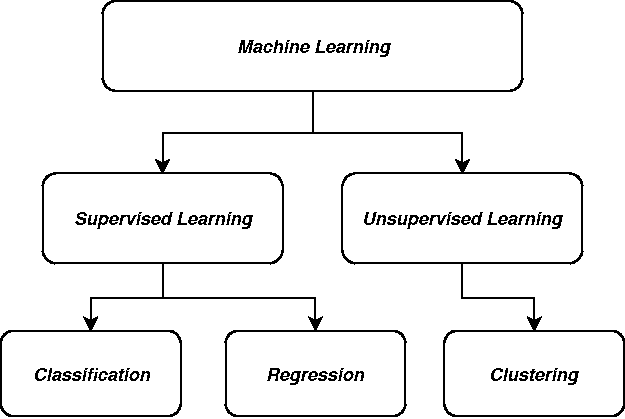
\includegraphics[width=10cm]{ML_hierachy.pdf}
	\caption{Hierarchy of Machine Learning methods}
	\label{mlHierachy}
\end{figure}

Before delving into methods for stance detection it is helpful to briefly review the topic of machine learning. Broadly speaking, this the process of computationally inferring a solution to a problem using past experience \cite{alpaydinIntroductionMachineLearning2014}. We take some prior knowledge (a\textbf{dataset}), extract relevant information (the \textbf{features}) and define a programmatic goal to be achieved (the \textbf{objective function}). We then iteratively train a program to identify patterns in the data (by \textbf{optimization} of the objective function), leading to a\textbf{ model }of the dataset. The model can be used to make predictions in future data, or to provide descriptions of existing data\cite{alpaydinIntroductionMachineLearning2014}. There are many forms of machine learning (figure \ref{mlHierachy}), but we can group them by the amount of `supervision' they receive in training \cite{geronHandsonMachineLearning2017}. All models in this project were achieved using supervised learning methods, so this review concentrates on supervised learning and considers other categories such as unsupervised, semi-supervised and reinforcement learning out of scope.

\subsection{Supervised Learning}
In the domain of supervised learning, each instance within our dataset includes the desired output (the \textbf{target variable}) \cite{geronHandsonMachineLearning2017}. In formal notation, for supervised learning we require that a dataset $ \mathcal{D}$ of size $N$ is specified by $ \mathcal{D} = \{(\mathbf{x}_i, y_i) | i = 1:N\}$, where $ \mathbf{x}_i \in \mathcal{X} $ represents an instance in the input space $ \mathcal{X} $ and $ y_i \in \mathcal{Y}$ is the associated target variable in the target space $ \mathcal{Y} $. We seek to learn a classifier $ \gamma $ that maps inputs to outputs:
$$ \gamma: \mathcal{X}\rightarrow\mathcal{Y}$$ 

The learning process is `supervised' during training by evaluating the quality of model output against an exact solution: correct predictions are rewarded and incorrect predictions are penalised via an optimization process such as stochastic gradient descent \cite{mendelsonAdvancedLecturesMachine2003}. Supervised learning includes both numeric prediction (regression), where the target variable is continuous, and classification, where the target variable is categorical \cite{wittenDataMiningPractical2011}. Since this project concerns a text classification task, this review is focussed on classification, with other kinds of supervised learning considered out of scope. 

\section{Text Classification}


\begin{figure}

	\centering
	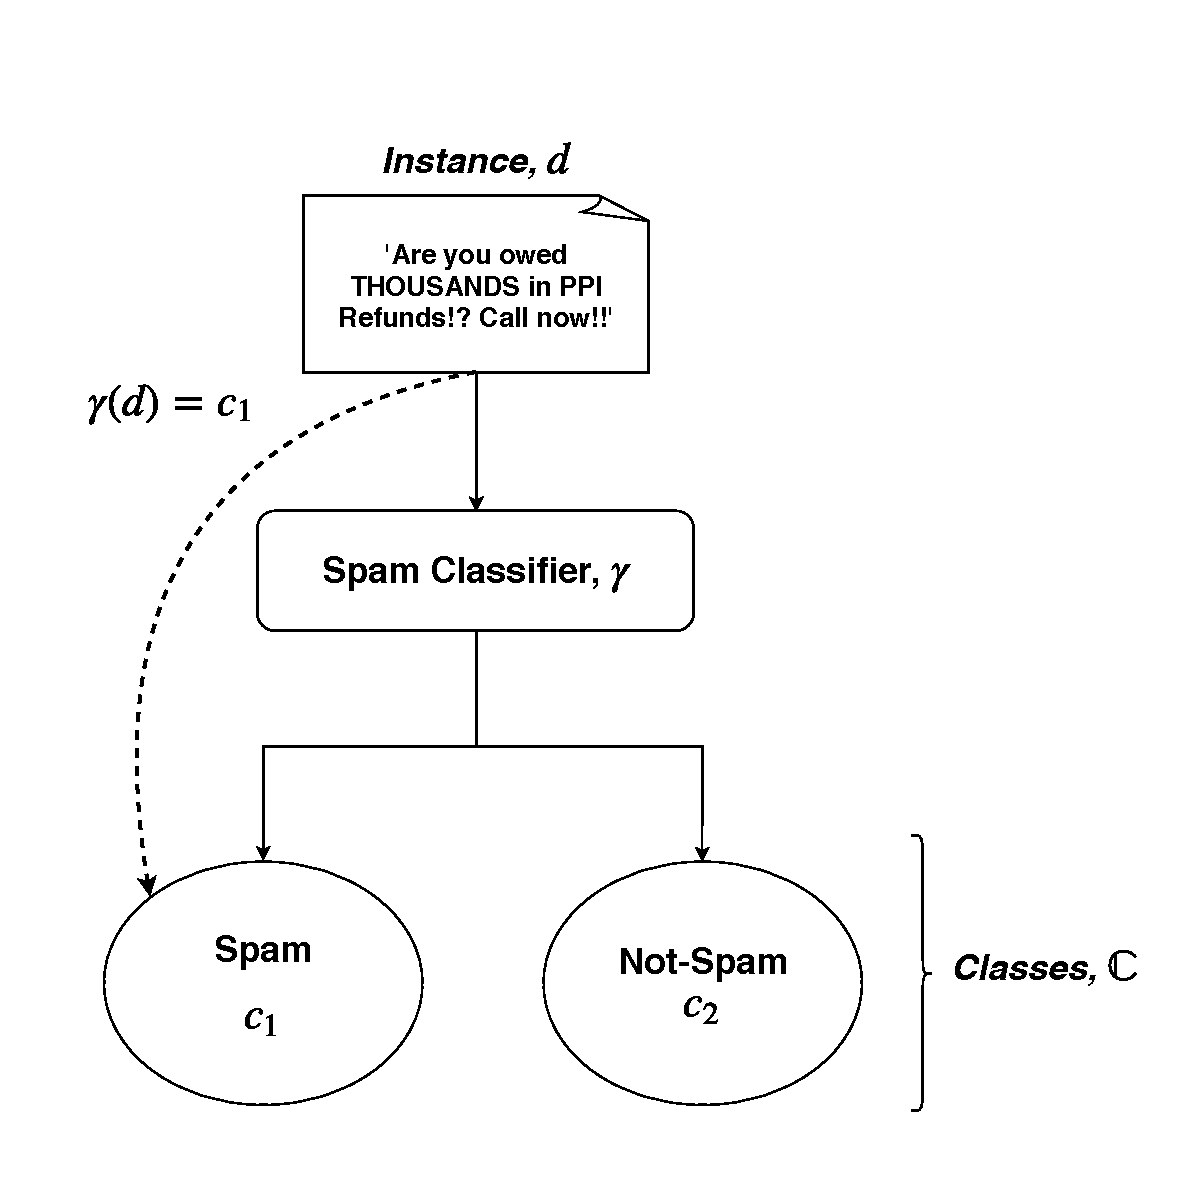
\includegraphics[width=11cm]{Spam_classifier.pdf}
	\caption{Simple spam classifier flowchart}
	\label{spamClassifier}
\end{figure}
Text Classification is a supervised learning, classification task in which we seek to assign a label, class or category to a word, sentence, text or document \cite{jurafskySpeechLanguageProcessing}. It has much importance in the fields of Information Retrieval and other areas of Natural Language Processing  as highlighted ing Manning, Raghavan and Sch\"{u}tze \cite{manningIntroductionInformationRetrieval2009}.
An example of text classification is flagging unwanted spam emails \cite{geronHandsonMachineLearning2017}. The dataset might consist of a collection of emails, with each instance entailing the textual contents of an email, associated metadata and a label of `spam` or `not-spam' \cite{geronHandsonMachineLearning2017}. The objective would be to learn a model that can accurately classify new incoming emails accordingly as `spam' or `not-spam'(see figure \ref{spamClassifier}). 

\subsection{Formal Definition}
In text classification we are given a document $ d \in \mathcal{X}$ where $ \mathcal{X} $ is the input document space, and  a set of disjoint classes $ \mathbb{C} = \{c_1,c_2,\dots c_j\}$  \cite{manningIntroductionInformationRetrieval2009}. The document space is generally some form of high dimensional feature space, while the classes are usually pre-defined natural language labels such as `spam' and `not-spam' as in figure~\ref{spamClassifier}\cite{manningIntroductionInformationRetrieval2009}. We have a dataset $\mathcal{D}$ of labelled instances $(d,c) \in \mathcal{X}\times \mathbb{C}$ and we seek to learn a classification function $ \gamma $ that maps inputs to classes \cite{manningIntroductionInformationRetrieval2009}:

$$
\gamma: \mathcal{X}\rightarrow \mathbb{C}
$$

We denote the \textit{learning method} as $ \Gamma $ such that $ \Gamma(\mathcal{D})= \gamma $ \cite{manningIntroductionInformationRetrieval2009}. The learning method applied to the dataset returns the classifier.  If $ |\mathbb{C}| = 2 $, then the classifier is performing \textit{binary classification}, which is a special case of the more general domain of \textit{multi-class classification}, where $ |\mathbb{C}| > 2 $ \cite{manningIntroductionInformationRetrieval2009}.


\subsection{Multi-Label Classification}\label{multiLabel}
In the previous sections we have considered \textit{single-label classification}, in which we assume  that for each instance there is only one correct label from the set of classes $ \mathbb{C} $. However, there are many situations in which this assumption does not hold, and we wish to assign to each instance a set of labels, $ \mathbf{y} = \{y_1,\ y_2,\  \dots, \ y_k\} \subseteq \mathbb{C}\} $ \cite{tsoumakasMiningMultilabelData2009}. This is known as \textit{multi-label classification}. For example, if we consider a hypothetical film genre classifier, we might want to label a film both as 'Action' and 'Thriller' or 'Romantic' and 'Comedy'. The Brexit Blog Corpus \cite{simakiAnnotatingSpeakerStance2017} provides a multi-label dataset, so it is important for the purpose of this project to review material concerning multi-label classification.

%\subsubsection{Problem Transformation Methods}
There exist a number of methods to transform multi-label datasets into forms that allow the application of traditional single-label classifying algorithms. Sorrower \cite{sorowerLiteratureSurveyAlgorithms2018} provides a useful review of such methods, some of which we will outline below. Certain methods such as \textit{select-max}, \textit{select-min} and \textit{select-random} extract only a single-label from each instance, while the \textit{ignore} method ignores all instance with more than one label \cite{sorowerLiteratureSurveyAlgorithms2018}. However, such methods do not provide fidelity with respect to the original dataset, and so are not considered further in this review. 

Of particular interest to this review are the \textit{label power set} and \textit{binary relevance} methods \cite{sorowerLiteratureSurveyAlgorithms2018}. To illustrate these methods Sorower \cite{sorowerLiteratureSurveyAlgorithms2018} considers a small data set, where four instances each belong to at least one class from the set $\mathbb{C} = \{c_1, \ c_2, \ c_3, \ c_4\}$ (see Table \ref{miniData}, part (a)).  In the label power set transformation each unique set of labels in the data is considered a single class in the transformed data \cite{sorowerLiteratureSurveyAlgorithms2018}. Thus, the problem can now be solved by a single-label classifier.

In the binary relevance method, $ k $ copies of the original dataset are created, where $ k = |\mathbb{C}| $. Each dataset is associated with one label $c_i \in \mathbb{C}$ with instances belonging to $ c_i $ labelled positively and all others labelled negatively (see Table \ref{miniData} part (c)). The target variable for each data set is therefore a binary variable, hence separate binary classifiers may be trained on each dataset and the results aggregated to provide the multi-label output \cite{sorowerLiteratureSurveyAlgorithms2018}.	

 
		
\begin{table}[]
	\centering

	\caption{Sample dataset in multi-label and label power set formats}
	\label{miniData}
	\begin{subfigure}{0.25\linewidth}
		\centering
		\subcaption{Original format}
		\begin{tabular*}{1\linewidth}{@{}cc@{}}
	
			\toprule
			Instance & Labels \\ \midrule
			1	&	$ \{c_2,c_3\} $        \\
			2	&	$ \{c_1\} $        \\
			3	&	$ \{c_1,c_2,c_3\} $        \\
			4	&	$ \{c_2, c_4\} $        \\ \bottomrule
		\end{tabular*}
	\end{subfigure}
	\qquad
	\begin{subfigure}{0.25\linewidth}
		\centering
		\subcaption{Label power set }
		\begin{tabular*}{1\linewidth}{@{}cc@{}}
			
			\toprule
			Instance & Label \\ \midrule
			1	&	$ c_{2,3} $        \\
			2	&	$ c_1$        \\
			3	&	$ c_{1,2,3} $        \\
			4	&	$ c_{2,4} $        \\ \bottomrule
		\end{tabular*}
	\end{subfigure}

\vspace{3ex}

	\begin{subfigure}{1\linewidth}
		\centering
		\subcaption{Binary relevance format}			
			\begin{subfigure}{0.2\linewidth}
				\subcaption*{$ c_1 $}
				\begin{tabular*}{1\linewidth}{@{}cc@{}}
					\toprule
					Instance & Label \\ \midrule
					1	&	0        \\
					2	&	1        \\
					3	&   1 	    \\
					4	&   0	    \\ \bottomrule
				\end{tabular*}
			\end{subfigure}
			\quad
			\begin{subfigure}{0.2\linewidth}
				\subcaption*{$ c_2 $}
				\begin{tabular*}{1\linewidth}{@{}cc@{}}
					\toprule
					Instance & Label \\ \midrule
					1	&	1        \\
					2	&	0        \\
					3	&	1        \\
					4	&	1        \\ \bottomrule
				\end{tabular*}
			\end{subfigure}
			\quad
			\begin{subfigure}{0.2\linewidth}
				\subcaption*{$c_3$}
				\begin{tabular*}{1\linewidth}{@{}cc@{}}
					\toprule
					Instance & Label \\ \midrule
					1	&	1        \\
					2	&	0        \\
					3	&	1        \\
					4	&	1        \\ \bottomrule
				\end{tabular*}
			\end{subfigure}
			\quad
			\begin{subfigure}{0.2\linewidth}
				\subcaption*{$ c_4 $}
				\begin{tabular*}{1\linewidth}{@{}cc@{}}
					\toprule
					Instance & Label \\ \midrule
					1	&	0        \\
					2	&	0        \\
					3	&	0        \\
					4	&	1        \\ \bottomrule
				\end{tabular*}
			\end{subfigure}
		\end{subfigure}

	
	
\end{table}


\subsection{Multi-Task Classification}
\section{Features and Embeddings}
\subsection{Vector Space Model and Feature Functions}\label{sec:vecSpace}


\begin{table}[]
	\caption{Simple Bag-of-Words example using term frequency weighting}
	\label{bagOfWords}
	\centering
	\begin{tabular}{@{}lllllllll@{}}
		\toprule
		& and                    & cat                    & eggs                   & green                  & ham                    & hat                    & in                     & the                    \\ \midrule  \cline{2-9} 
		\multicolumn{1}{l|}{`the cat in the hat'} & \multicolumn{1}{c|}{0} & \multicolumn{1}{c|}{1} & \multicolumn{1}{c|}{0} & \multicolumn{1}{c|}{0} & \multicolumn{1}{c|}{0} & \multicolumn{1}{c|}{1} & \multicolumn{1}{c|}{1} & \multicolumn{1}{c|}{2} \\ \cline{2-9} 
		\multicolumn{1}{l|}{`green eggs and ham'} & \multicolumn{1}{c|}{1} & \multicolumn{1}{c|}{0} & \multicolumn{1}{c|}{1} & \multicolumn{1}{c|}{1} & \multicolumn{1}{c|}{1} & \multicolumn{1}{c|}{0} & \multicolumn{1}{c|}{0} & \multicolumn{1}{c|}{0} \\  \cline{2-9} 
		&                        &                        &                        &                        &                        &                        &                        &                        \\ \bottomrule
	\end{tabular}
	
\end{table}

In text classification we face the problem of how best to represent the input data, since machine learning models generally require natural numbers as inputs. A common method for this in information retrieval is the vector space model as proposed by Salton, Wong and Yang \cite{saltonVectorSpaceModel1975}. In their vector space model a document in a collection $ D_i $ is represented by a $ t $ dimensional vector of term weights: $$ D_i = (d_{i1},\ d_{i2},\ \dots,\ d_{ij})  $$ where $ t $ is the magnitude of the vocabulary present in the document collection and $ d_{ij} $ is the weight value for the $ j^{th} $ term in the $ i^{th} $ document \cite{saltonVectorSpaceModel1975}.
The order of words is not considered, only the presence and the frequency. This is known as the Bag-of-Words model (see Table \ref{bagOfWords}) \cite{jurafskySpeechLanguageProcessing}. The term weight value is determined by a weighting scheme. Common weighting schemes are binary, term-frequency and tf-idf.

In binary term weighting each term weight $ d_{ij} $ is a binary indicator taking the value of either 0 or 1 to indicate the presence of the $ j^{th} $ term. Term frequency is ignored. This is analogous to One-Hot-Encoding in which categorical variables such as gender are converted to real numbers as a vector of binary indicators, with one indicator per variable category \cite{geronHandsonMachineLearning2017}.

In term-frequency weighting each term weight is determined as $d_{ij} = tf_{ij}$ where $tf_{ij}$ is the frequency of the $ j^{th}$ term in the $i^{th}$ document. However, this introduces a large bias towards frequent terms such as \{\textit{the, I, you}\} which often encode little to no semantic information \cite{manningIntroductionInformationRetrieval2009}.

Tf-idf avoids this bias by weighting each term frequency by the \textit{inverse document frequency} which is defined by Manning et al.\ \cite{manningIntroductionInformationRetrieval2009} as:

$$idf_j = log \frac{N}{df_j} $$

Where $ N $ is the number of documents in the collection and $ df_j $ is the number of documents that contain the $ j^{th} $ term. Hence, we can see that the tf-idf weight of common terms will be attenuated by a low idf, and conversely rare terms (which encode greater semantic information) will have their weights boosted by a high idf \cite{manningIntroductionInformationRetrieval2009}.

Here by examining the vector space model we have conveniently introduced the concept of a feature function that produces a feature vector. Often denoted by $ \phi() $ or $ \phi(\mathbf{x}) $,  with careful selection and tuning the feature selection process can help to increase the discriminating power of our classifier \cite{bishopPatternRecognitionMachine2006}. Bishop \cite{bishopPatternRecognitionMachine2006} highlights that we can take advantage of domain specific knowledge to develop effective feature functions. For example in text classification we might wish to use a feature function that concatenates the Bag-of-Words representation with other semantic or syntactic features under the intuition that such extra information might increase classifier performance. 

\subsection{Vector Semantics and Word Embeddings}
\begin{figure}[h]
	\centering
	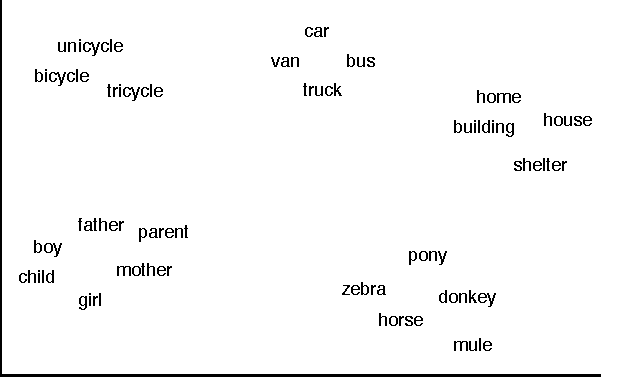
\includegraphics[width=4in]{word_embeddings.pdf}
	\caption{Visualisation of word embeddings in 2-D
		\label{fig:wordEmbeds} space}
\end{figure}

Section \ref{sec:vecSpace} briefly introduces the vector space model and highlights the importance of feature extraction for textual data. While simple N-gram bag of words models are conceptually simple and generally effective, such approaches suffer from two importatn problems. Firstly, words are treated as atomic units and no semantic similarity is captured in the feature representation. Secondly, when using large training vocabularies feature vectors become very sparse: in an N-gram model feature dimensionality scales as $ |V|^N $ where $ N $ is gram length and $ |V|  $ is the size of vocabulary.  The complete Oxford English Dictionary alone contains nearly 250,000 words \cite{HowManyWords} without taking account of technical terms, dialects and regional spelling variation, so it is clear that any suitably large training corpus will result in incredibly sparse representations \cite{jurafskySpeechLanguageProcessing}. The limitations of such sparse feature representations can however be avoided by using vector semantics and dense word embeddings \cite{jurafskySpeechLanguageProcessing}.

The distributional hypothesis  posits that words appearing in similar contexts have similar meanings \cite{sahlgren2008distributional}. Vector semantics aims to capture this similarity by representing words as dense vectors embedded in a multidimensional space, which are learned from the distributions of words and contexts in corpora \cite{jurafskySpeechLanguageProcessing}. This is known as representation learning, where we generate representation of text by unsupervised learning instead of feature engineering \cite{jurafskySpeechLanguageProcessing}. Figure \ref{fig:wordEmbeds} shows an extract of what a word vector embedding space might look like projected into two dimensions. Notice that semantically similar words are specially grouped. There are several popular formats for word embeddings including skip-gram (word2vec) \cite{mikolovEfficientEstimationWord2013}, GloVe \cite{penningtonGloveGlobalVectors2014} and fastText \cite{joulinBagTricksEfficient2016}, though there are broad similarities between all three methods. A key innovation in this field was the use of running text as implicitly supervised training data - any given sentence already contains the target variable for a classifier that predicts the next word in a sentence \cite{jurafskySpeechLanguageProcessing}. In particular, a neural language model that accomplishes this will learn a weight matrix from which embedded word representations can be extracted \cite{jurafskySpeechLanguageProcessing}. 

\section{Classifers}
This section reviews relevant material concerning the classifiers used throughout this project. Classifier choice can play a significant role in model performance, so it is important to ensure the choice is appropriate for the task at hand.
\subsection{Logistic Regression}

\begin{figure}
	\centering
	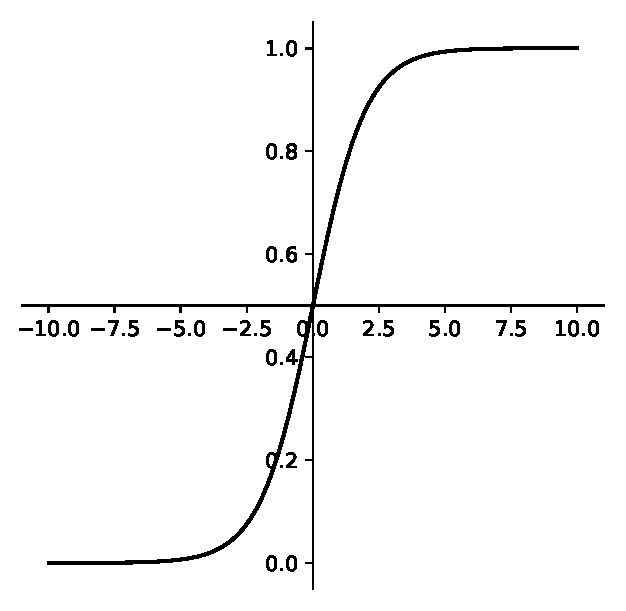
\includegraphics[width=3in]{sigmoid.pdf}
	\caption{Logistic sigmoid function}
	\label{logisticFunction}
\end{figure}
Logistic regression is part of a family of classifiers known as linear classifiers.	Bishop \cite{bishopPatternRecognitionMachine2006} provides a comprehensive overview of linear classifiers and defines the simplest general form as follows:

$$ 
 y(\mathbf{x}) = f(\mathbf{w}^\top\mathbf{x}) 
$$

Here $ y $ is the classifier prediction, $ \mathbf{x} $ is the input data vector, $ \mathbf{w} $ is a learned parameter vector and $ f(\cdot) $ is an \textit{activation function} - a nonlinear transformation that maps unbounded real numbers to probabilities in the range \{0,1\}. Specifically in logistic regression we introduce the \textit{logistic sigmoid} activation function, defined in  \cite{bishopPatternRecognitionMachine2006} as:

\[ \sigma(a) = \frac{1}{1 + \mathrm{exp}(-a)} \]

Therefore, with the inclusion of a feature function $ \phi(\cdot) $ binary logistic regression with classes $ \mathbb{C} = \{c_1, c_2\} $ \cite{bishopPatternRecognitionMachine2006} defines the probability of a positive label as:

\[ \mathrm{P}(c_1|\phi(\mathbf{x})) = y(\phi(\mathbf{x})) =  \sigma(\mathbf{w}^\top\phi(\mathbf{x}
)) \]

It follows that the probability of the negative label is given by: $$ \mathrm{P}(c_2| \phi(\mathbf{x})) = 1-\mathrm{P}(c_1|\phi(\mathbf{x})) $$

Logistic regression can also be generalized to multi-class domains where $ \mathbb{C} = \{c_1,\ c_2\, \ \dots,\ c_j \} $:

\[ \mathrm{P}(c_k|\phi(\mathbf{x})) = y_k(\phi(\mathbf{x})) =  \frac{\mathrm{exp}(a_k)}{\sum_{j}\mathrm{exp}(a_j)}   \]

Where the activation $ a_k $ is given by:
 \[a_k =  \mathbf{w}_k^\top\phi(\mathbf{x})  \]
 
In order to use logistic regression in a multi-label context the binary relevance transformation described in section \ref{multiLabel} must be used and multiple binary logistic regression classifiers thereby trained.

\subsection{Neural Networks}
\begin{figure}[h]

	\centering
	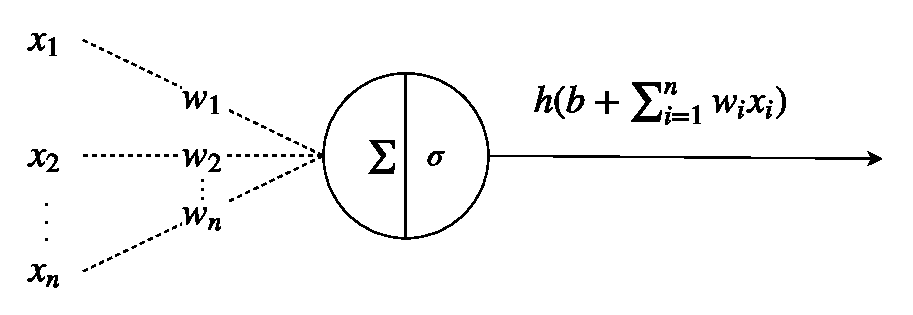
\includegraphics[width=5in]{neuron.pdf}

	\caption{Artificial neuron}
	\label{fig:neuron}
\end{figure}

\begin{figure}
	\centering
	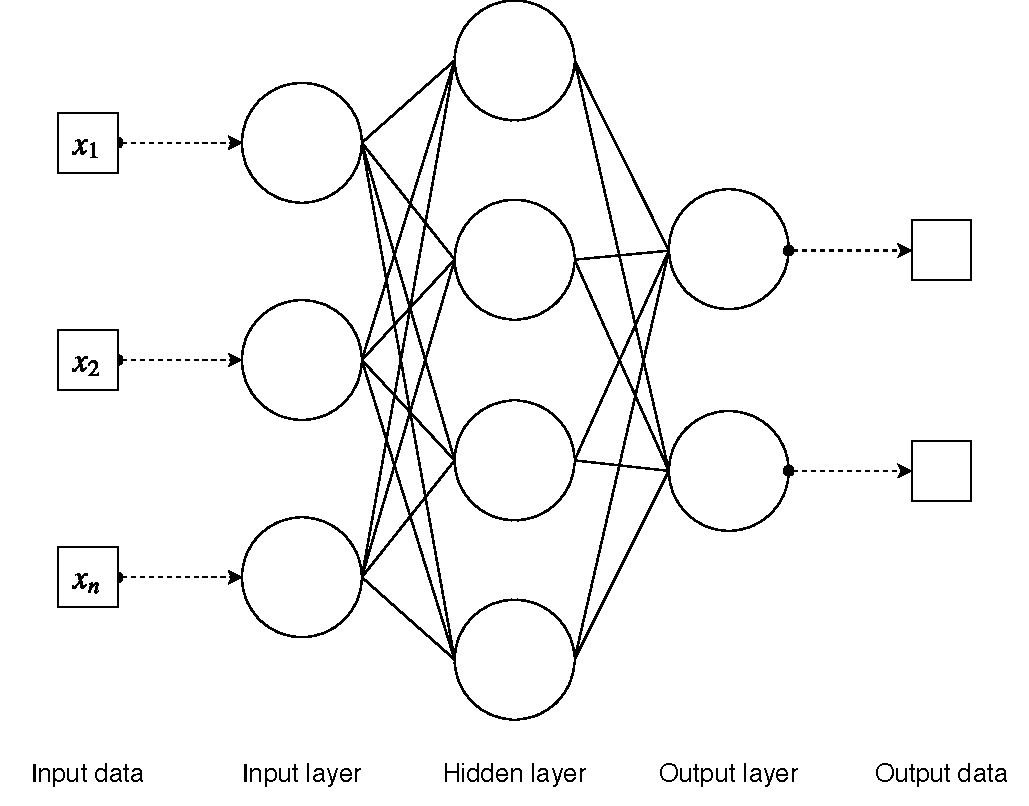
\includegraphics[width=5in]{simple_NN.pdf}
	\caption{Simple multilayer perceptron}
	\label{fig:multilayerPercep}
\end{figure}

In recent years there has been a resurgence in interest amongst researchers about neural networks and deep learning. First investigated in the 1950s, current technological advancements have lead to enourmous growth in performance and scalability of neural networks \cite{pattersonDeepLearningPractitioner2017}. In particular, neural networks have shown great promise and versatility in many natural language processing tasks. This section reviews the basic elements to neural networks and certain architectures that are used in the approach to stance detection presented by this project. 

The basic unit of a neural network is the artificial neuron (see Figure \ref{fig:neuron}). Each neuron maps a vector of inputs to a single output by a non linear activation function $ h(\cdot) $ \cite{pattersonDeepLearningPractitioner2017}. The activation $ a_k $ of a neuron receiving inputs $ \mathbf{x} = \{x_1,x_2,\ \dots,\ x_n\} $ is defined by \cite{pattersonDeepLearningPractitioner2017}:

\[ a_k = h(b + \sum_{i=1}^n w_ix_i) \]

Where $ b $ and $ \mathbf{w} = \{w_1,w_2, \ \dots, \ w_n\} $ are learned parameters. Common activation functions include the logistic sigmoid (see Figure \ref{logisticFunction}) and the rectified linear unit function (ReLU)(see Figure \ref{fig:ReLU}).

\begin{figure}
	\centering
	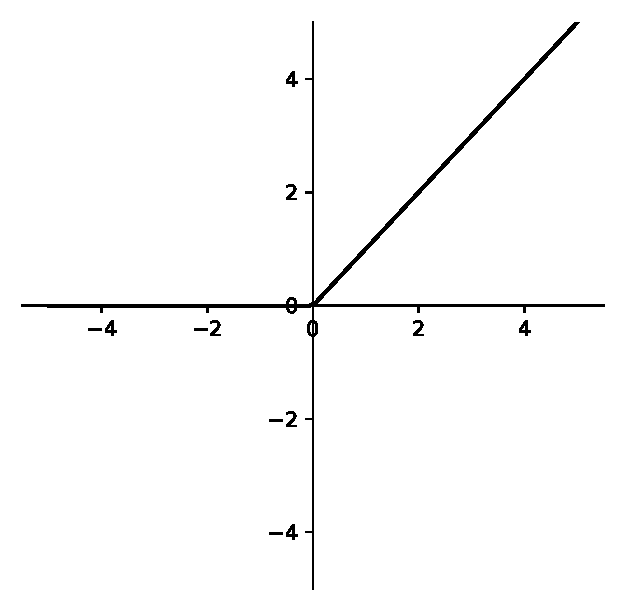
\includegraphics[width=3in]{ReLu.pdf}

	\caption{ReLU activation function}
	\label{fig:ReLU}

\end{figure}

Neural networks are structured in layers of neurons, the connectivity between and within which defines the architecture of a network. In the simplest networks (known as multilayer perceptrons, see Figure \ref{fig:multilayerPercep}) each neuron is fully connected, taking input from every unit in the preceding layer and feeding forward the output activation to every unit in the following layer. \cite{pattersonDeepLearningPractitioner2017}. More complex architectures introduce semi-connected layers (Convolutional Neural Network) and recurrent layers (Recurrent Neural Networks)\cite{pattersonDeepLearningPractitioner2017}

\cite{jurafskySpeechLanguageProcessing}


\subsection{FastText}
\begin{figure}
	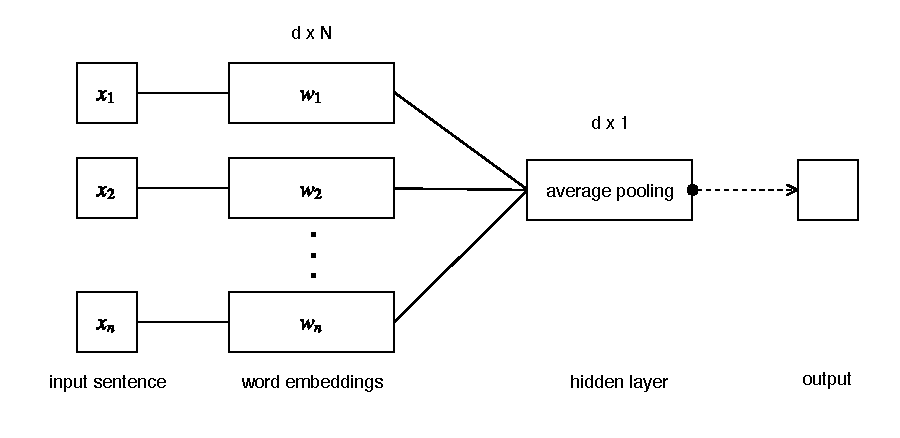
\includegraphics[width=5in]{fastText.pdf}
	\caption{FastText embedding architecture for $ d $-dimensional embedding and sentence length $ N $}
\end{figure}
\subsection{Anchors}
\section{Stance Detection}\label{stanceDetection}


	
\subsection{Commonalities and Differences with Sentiment Analysis}
\section{Previous Research in Stance Detection} \label{sec:priorWork}
In recent years there has been a wealth of research in the related fields of sentiment analysis and opinion mining, coinciding with an explosion of opinionated user generated online content \cite{liuSentimentAnalysisOpinion}. Like sentiment analysis and opinion mining, stance detection inherently concerns opinionated content and as such datasets presented for the task usually focus on online debate, micro-blogging and journalism. However, stance detection remains a fairly novel niche within natural language processing and so the variety of public datasets used is limited, with the two most common being the annotated twitter datasets presented for the shared tasks of The Fake News Challenge \cite{FakeNewsChallenge} and SemEval Task 6: Detecting Stance in Tweets \cite{TaskDetectingStance} (hereafter, SemEval). Stance detecton is frequently presented in context of second task. The Fake News Challenge suggests stance detection as a preliminary step in fake news identification, while Ferreira and Vlachos consider stance detection as part of a wider set of natural language processing tasks used for fact-checking \cite{ferreiraEmergentNovelDataset2016} and Mohammad et al.\ \cite{mohammadStanceSentimentTweets2016} explores the relationship between sentiment analysis and stance detection. Finally, Respall and Derczynski \cite{respallStanceDetectionCatalan} focusses on stance detection and author gender identification.

Previous work tends to consider English language Twitter data and use tertiary classification with the labels \{\textit{Favour, Against, Neither}\} as in \cite{TaskDetectingStance,mohammadStanceSentimentTweets2016,mohammadSemEval2016TaskDetecting2016,augensteinStanceDetectionBidirectional2016,deyTwitterStanceDetection2017,deyTopicalStanceDetection2018}. The Fake News Challenge \cite{FakeNewsChallenge} also uses English language twitter data but distinguishes between neutral content topically related to the target and unrelated content with the classes \{\textit{for, against, discusses, unrelated}\}. Swami \cite{swamiEnglishHindiCodeMixedCorpus2018} uses the tertiary classification labels on a dataset of code-mixed\footnote{The mixing of two or more languages in speech or text by multilingual interlocutors} Hindi-English tweets. Du et al.\  \cite{duStanceClassificationTargetspecific} again uses tertiary classification, however they demonstrate the language independence of their approach by using an English twitter dataset and a Chinese Weibo\footnote{Chinese micro-blogging platform similar to Twitter} dataset.  Respall and Derczynski \cite{respallStanceDetectionCatalan} use a dataset consisting of Spanish and Catalan tweets annotated again in the tertiary labelling scheme. Ferriera and Vlachos \cite{ferreiraEmergentNovelDataset2016} present Emergent, a novel dataset that consists of 2,595 English news article headlines labelled according to the stance they take with respect to 300 target claims under a tertiary classification scheme of \{\textit{For, Against, Observing}\}.

In terms of the approaches taken to stance detection, the literature is split between feature engineering approaches and neural, representation learning approaches. Below these methods are outlined to provide context for this project in terms of what the current state of the art includes.

.......................................

Mohammad et al.\ \cite{mohammadStanceSentimentTweets2016} is a seminal work in the stance detection literature. \cite{mohammadStanceSentimentTweets2016} introduces twitter the dataset used in SemEval \cite{TaskDetectingStance}, consisting of tweet

.....................................

Mohammad et al.\ \cite{mohammadSemEval2016TaskDetecting2016} provides a retrospective summary of SemEval \cite{TaskDetectingStance} . Within SemEval \cite{TaskDetectingStance} were two subtasks, task A and task B. Task A tested stance detection on tweets associated with five target topics: athiesm, climate change, feminism, Hillary Clinton and abortion with in  a supervised learning framework. The highest ranking submission at the time of publication, MITRE, developed a semi-supervised approach that stacks two RNNs, achieving an overall macro averaged F-score of 67.82. However, this did not beat the n-gram Support Vector Machine (SVM) Baseline created by the task organisers. Task B tested stance in tweets towards Donald Trump, however the training data provided was unlabelled for stance. The winning system at time of publication, pkudblab, used a weakly supervised approach that used a rule based annotation of the unlabelled training data to augmented a deep convolutional network, achieving an overall macro averaged F-score of 56.28.

Augenstein et al.\ \cite{augensteinStanceDetectionBidirectional2016} publishes a post-hoc method for SemEval task B \cite{TaskDetectingStance}, developing a method known as bi-directional conditional encoding. Encoding refers to generating separate representations of tweets and target topics using two LSTMs \cite{augensteinStanceDetectionBidirectional2016}\cite{hochreiterLongShorttermMemory1997}. Conditional encoding improves upon this by initializing the tweet LSTM with the state of the target LSTM, thereby generating a target dependent representation of each tweet \cite{augensteinStanceDetectionBidirectional2016}. Finally, Bi-directional means that the conditional encoding process is performed reading the text both left to right and right to left to enhance the representation and improve performance \cite{augensteinStanceDetectionBidirectional2016}. The approach results in a macro averaged F-score of 49.01 when using the unlabelled training data, and 58.03 when using a weakly supervised approach similar to that of the winning SemEval submission, pkudblab.


Dey et al.\ \cite{deyTwitterStanceDetection2017} provides another post-hoc approach to SemEval, but for task A. The method uses feature engineering and a two phase SVM classifier. The first phase seperates neutral tweets from non-neutral using WordNet \cite{WordNetLexicalDatabase} features and a subjectivity-polarity score from the MPQA subjectivity lexicon \cite{SubjectivityLexiconMPQA} (MPQA). The second phase then differentiates between Favour and Against tweets using MPQA and SentiWordNet \cite{SentiWordNet} features, character and word n-grams, frame semantics and boolean indicators for the presence of target words in tweets. This approach nets a macro averaged F-score of 69.53, and thus represents the current state of the art with respect to SemEval task A.

Du et al.\ \cite{duStanceClassificationTargetspecific} introduces a novel application of neural attention networks for the purpose of stance detection. In the neural attention network an attention signal is learned. The signal is multiplied with instance features effectively highlighting critical elements of text in relation to a target topic and masking unimportant elements. This mechanism is incorporated into a bi-directional RNN that achieves a macro averaged F-score of 68.79 on SemEval task A, and 72.88 on a Chinese dataset.

Dey et al.\ return to the SemEval problem in \cite{deyTopicalStanceDetection2018}, this time publishing a two phase LSTM method that incorporates the attention mechanism of \cite{duStanceClassificationTargetspecific}. This method achieves a macro averaged F-score of 68.84 on SemEval, currently representing the state of the art for this task.


The work of Ferriera and Vlachos \cite{ferreiraEmergentNovelDataset2016} on the Emergent datasets uses a logistic regression classifier and a feature space combining simple headline linguistic features such as Bag-of-words and punctuation with headline-claim features such as alignment, entailment and cosine similarity, achieving a test set accuracy of 73\%.


......................

Need to find paper from Fake News Challenge

......................
	\section{The Brexit Blog Corpus}\label{BBC}


Simaki et al.\ \cite{simakiAnnotatingSpeakerStance2017} introduces The Brexit Blog Corpus, a novel dataset annotated for speaker stance. The work is undertaken in the field of corpus linguistics and linguistic theory, and therefore uses a much richer operational definition of stance (as outlined in section \ref{sec:speakerStanceLing}) compared to work published in machine learning journals. Simaki et al.\ \cite{simakiAnnotatingSpeakerStance2017} acknowledges this, justifying that their approach offers much more context sensitivity than traditional simple lexically driven approaches. In section \ref{sec:priorWork} it is noted that most work considers stance detection as a single-label, tertiary classification task, however \cite{simakiAnnotatingSpeakerStance2017} introduces a labelling scheme comprising ten stance categories as per Table \ref{tab:stanceCats}. The dataset presents stance annotation as a multi-label classification problem, in contrast to previous work which only considers single-label classification schemes. 

{\renewcommand{\arraystretch}{1.5}
	\begin{table}[h]
	\centering
	\begin{tabular}{|l|l|}
		\hline
		Agreement/Disagreement & Certainty       \\ \hline
		Contrariety            & Hypotheticality \\ \hline
		Neccessity             & Prediction      \\ \hline
		Source of Knowledge    & Tact/Rudeness   \\ \hline
		Uncertainty            & Volition        \\ \hline
	\end{tabular}
	\caption{The 10 stance categories used in the Brexit Blog corpus \cite{simakiAnnotatingSpeakerStance2017}}
	\label{tab:stanceCats}
\end{table}}

This broader interpretation of \textit{stance} offers significant novelty and potential for natural language procession applications, however it also presents a much more complex problem space. At the time of writing, there exist no publications that apply stance classification methods to the Brexit Blog Corpus, and it is therefore an aim of this project to provide a preliminary baseline for subsequent stance detection research into the Brexit Blog Corpus.

\subsection{Quantitative Linguistic Analysis}
Simaki et al.\ \cite{simakiEvaluatingStanceannotatedSentences2018} examines a subset of The Brexit Blog Corpus for the purpose of formal quantitative analysis of linguistic characteristics. The subset comprises six out of the ten categories, and for each category normalised frequency values are obtained of 29 linguistic features such spaces, upper case letters etc. Simaki et al.\cite{simakiEvaluatingStanceannotatedSentences2018} then uses one-way Analysis of Variance (ANOVA) to establish which features exhibit significant differences in frequency between categories. discriminating linguistic features. The process identified 19 significant features for differentiating between the six stance categories.

\end{document}